\documentclass {article}

\usepackage[utf8]{inputenc}
\usepackage[T1]{fontenc}
\usepackage[francais]{babel}
\usepackage{layout}
\usepackage[top=1.5cm, bottom=1.5cm, left= 2cm, right=2cm]{geometry}
\usepackage{hyperref}
\usepackage{charter}
\usepackage{graphicx}

\title{Manuel utilisateur de MIST
\\
version 1.0
\\
\copyright Benjamin \bsc{gilles}}

\author{Valentin \bsc{favier}, Benjamin \bsc{gilles}}
\date{Juin 2016
\\
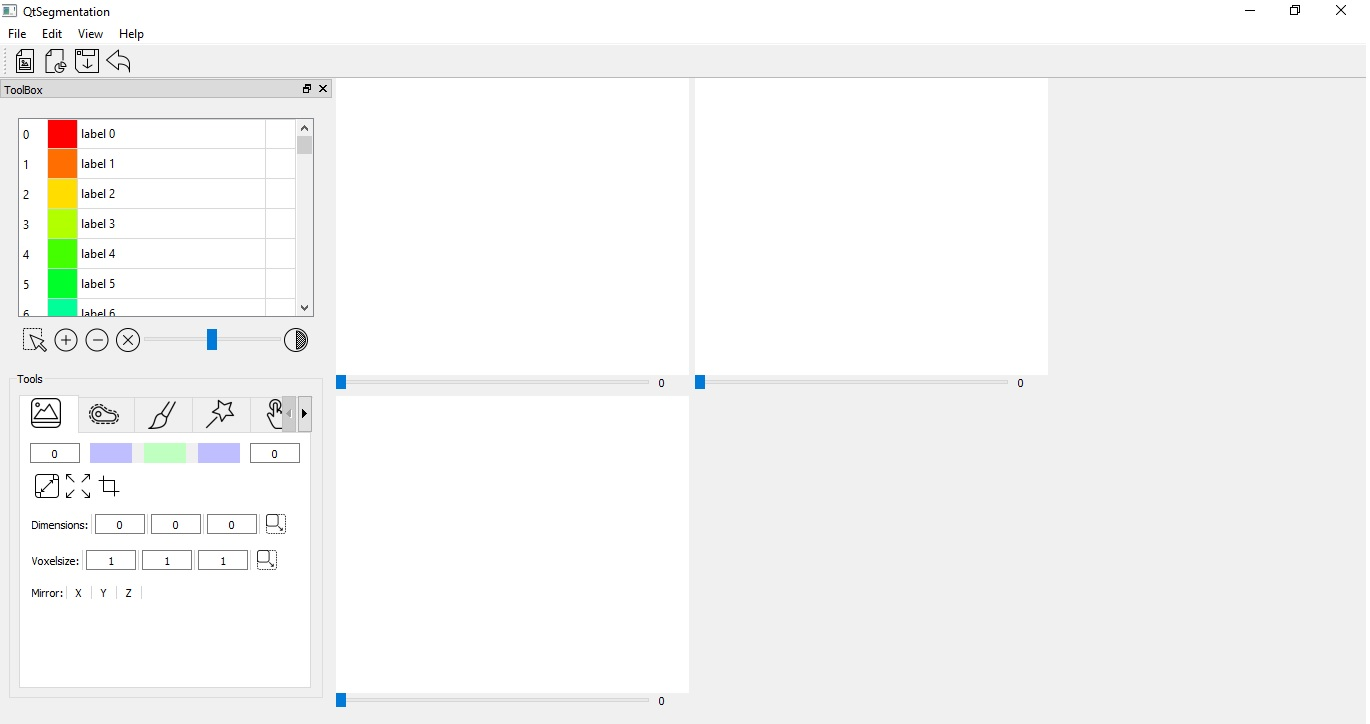
\includegraphics[scale=0.5]{Iconographie/Interface_vierge}}

				


\begin{document}

\maketitle
\newpage

\part{Introduction}

MIST est un logiciel en accès libre. C'est un outil manuel de segmentation d'images, proposant des fonctionnalités de base permettant d'aboutir à un maillage tridimensionnel.
\\
Cette documentation est destinée à permettre la prise en main du logiciel par les débutants en informatique et traitement d'image volumique.

\part{Installation de MIST}

\section{Programmes pré-requis}

Pour l'installation et la compilation du logiciel, les programmes suivants doivent être installés au préalable:
\begin{description}
\item[QT creator]: \url{https://www.qt.io/download/}
\item[Code source sur github]: \url{https://github.com/BenjaminGilles/MIST}
\end{description}

\section{Installation}

\part{Interface}

Lors de l'ouverture de MIST, l'interface s'affiche. 


	\begin{center}
				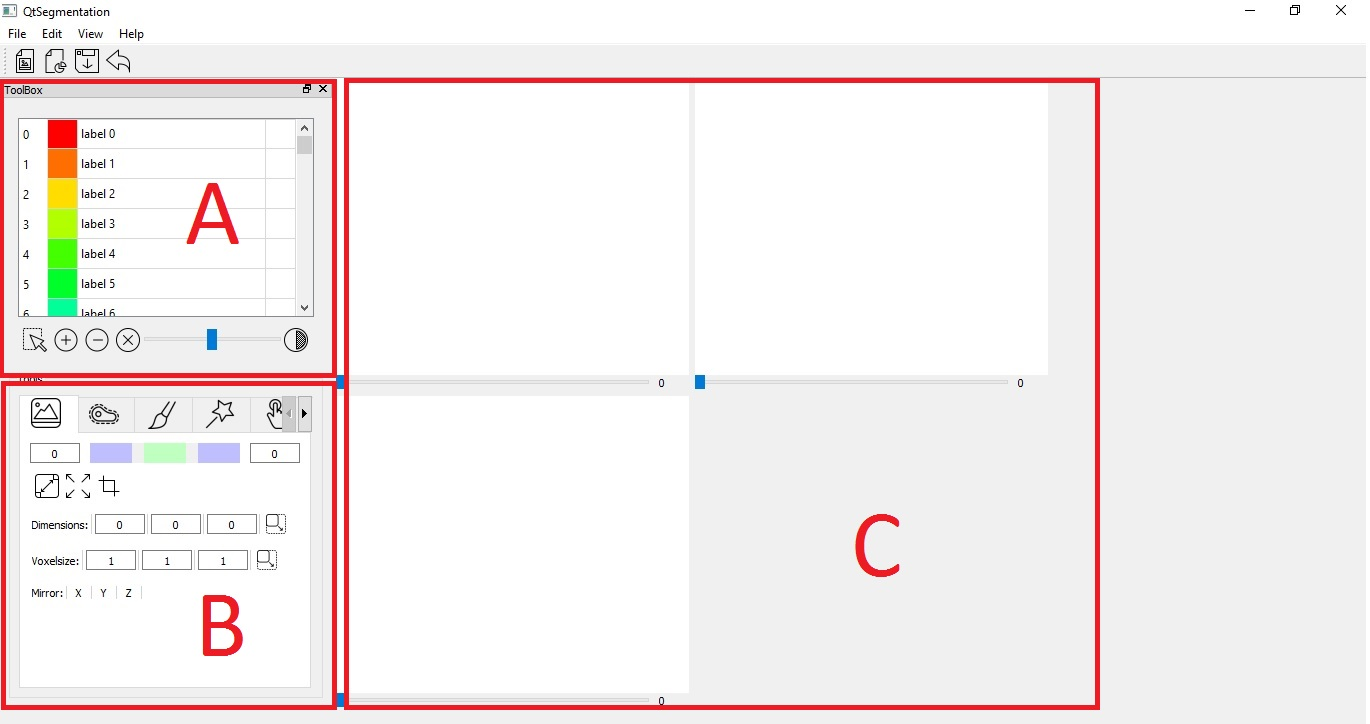
\includegraphics[scale=0.5]{Iconographie/Interface_fenetres}
	\end{center}



Elle est composée de 3 fenêtres et d'une barre des tâches.
\\
\textbf{Les fenêtres:}
\begin{itemize}
	\item[\textbf{A}]: Partie supérieure de la boîte à outils (toolbox) correspondant aux labels utilisés dans la segmentation. Un label désigne une sélection de points dans une image. Chaque image peut être segmentée en plusieurs labels. Ils sont définis par un nom et une couleur qui peuvent être personnalisés.
	\item[\textbf{B}]: Partie inférieure de la boite à outils (toolbox). Elle regroupe l'ensemble des opérations pouvant être effectuées sur les images. Un menu déroulant latéral permet de sélectionner les différentes familles d'outils. La toolbox dans son ensemble (fenêtre A + B) peut être déplacée ou supprimée de l'interface.
	\item[\textbf{C}]: C'est dans cette partie de l'interface que s'afficheront les images selon 3 plans: XY en haut à gauche, ZY en haut à droite et XZ en bas. Chacun de ces plans peut être désélectionné. Si vous souhaitez n'afficher qu'un seul plan, ce dernier sera automatiquement redimensionné à la taille de la fenêtre pour une meilleure visualisation.
\end{itemize}


\part{Prise en main}

Pour charger une image, cliquez sur l'onglet File puis Open Image. Raccourci clavier CTRL+O. Si vous avez à modifier l'image en elle même (après rognage par exemple) et que vous souhaitez l'enregistrer, cliquez sur File puis Save Image. Attention, cette manoeuvre enregistre l'image et non la segmentation!
\\
Pour commencer à segmenter, aucune autre étape n'est nécessaire. Vous aurez à sauvegarder la segmentation (File puis Save segmentation as...) dans un dossier spécifié. Les prochaines sauvegardes pourront être réalisées avec le raccourci clavier CTRL+S. Pour charger une segmentation sur laquelle vous avez déjà travaillé, cliquez sur File puis Open segmentation.
\\
L'onglet View permet d'afficher ou de désafficher les différentes fenêtres de l'interface: la toolbox et les différents plans de visualisation de votre image (XY, ZY, XZ).

\part{Fonctionnalités}

\section{Labels}

La partie haute de la toolbox (fenêtre A) renseigne sur les labels. 

\begin{center}
		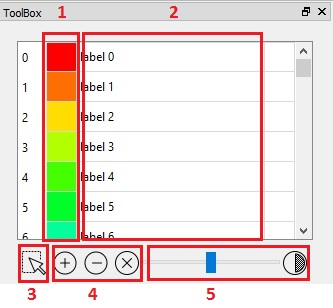
\includegraphics{Iconographie/toolbox_A}
\end{center}


Vous pouvez:
\begin{itemize}
	\item[\textbf{1}]: Changer la couleur du label en double cliquant sur la couleur
	\item[\textbf{2}]: Changer le nom du label en double cliquant sur le nom.  Il est également possible de verrouiller le label, en cliquant sur la case située à droite de son nom, afin que les changements effectués sur les autres labels n'empiètent pas sur celui-ci.
	\item[\textbf{3}]: Sélectionner l'ensemble des points faisant partie du label (ne concerne pas uniquement les points visibles sur la coupe sélectionnée mais tous les points du label sur l'ensemble des coupes)
	\item[\textbf{4}]: Lorsque des points sont sélectionnés, il est possible des les ajouter au label ((+) ou ENTER), de les soustraire au label ((-) ou RETURN) ou de les désélectionner ((X) ou ESPACE).
	\item[\textbf{5}]: Il est possible de faire varier la transparence de l'ensemble des labels sur l'image en déplaçant ce curseur. Le bouton situé à droite du curseur permet de varier l'affichage des labels: les contours seuls ou la forme pleine.
\end{itemize}

Les fonctions suivantes sont toutes disponibles dans la partie basse de la toolbox (fenêtre B).

\section{Image tools}

Ces outils permettent de retravailler l'image en elle-même (et non la segmentation!). Attention cependant à ne pas charger une segmentation après avoir retravaillé une image, cela risque de produire des incompatibilités.

\begin{itemize}
	\item[\textbf{1}]: permet de faire varier le contraste de l'image. Le double curseur renseigne sur le contraste minimal et le contraste maximal à afficher. Pour plus de précision il est possible de taper directement des données chiffrées dans les cases prévues à cet effet: contraste minimal dans la case de gauche, contraste maximal dans la case de droite.
	\item[\textbf{2}]: De gauche à droite: le premier bouton permet de sélectionner une région sur l'image pour l'agrandir (zoom in). Cette opération est annulable grâce au deuxième bouton (reset zoom). Si vous souhaitez rogner l'image (couper l'image au niveau de la sélection), il faut d'abord utiliser l'outil zoom in puis cliquer sur le troisième bouton (crop image). Attention, cette opération est définitive. L'intérêt de cette dernière opération est de s'affranchir de zones de l'image qui ne sont pas utiles au travail et qui ralentissent l'usage du logiciel. Pensez ensuite à sauvegarder l'image elle-même (File puis Save Image) une fois rognée.
	\item[\textbf{3}]: Il est possible de redimensionner directement l'image en renseignant les valeurs numériques correspondant aux côtés de l'image volumique.
	\item[\textbf{4}]: De même, il est possible de redéfinir la taille des voxels. Agrandir la taille des voxels diminue la résolution de la segmentation; diminuer leur taille permet d'augmenter la résolution de la segmentation. N'oubliez pas de sauvegarder l'image une fois les modifications effectuées. Attention à réaliser ces modifications d'image avant de débuter la segmentation.
	\item[\textbf{5}]: La fonction miroir permet de faire pivoter l'image de 180\degre selon un axe de symétrie X Y ou Z. N'oubliez pas de sauvegarder l'image une fois les modifications effectuées. Attention à réaliser ces modifications d'image avant de débuter la segmentation.
	
\end{itemize}
\section{Morphological operators}

Ces outils permettent de retravailler une sélection de points.

\begin{center}
			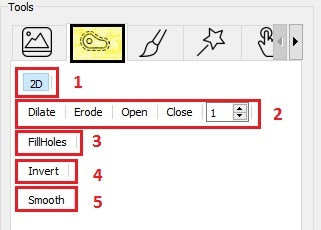
\includegraphics{Iconographie/morphological_operator.jpg}
\end{center}


\begin{itemize}
	\item[\textbf{1}]:	Option permettant d'effectuer la modification sur la sélection en 2D (uniquement sur la coupe affichée) ou en 3D (sur toutes les coupes). 
	\item[\textbf{2}]: De gauche à droite: dilatation de la sélection (augmentation de taille à partir de la périphérie de la sélection, selon le nombre de voxels prédéfinis), érosion de la sélection (diminution de taille à partir de la périphérie de la sélection, selon le nombre de voxel prédéfinis). Les opérations d'ouverture et de fermeture sont une combinaison des étapes de dilatation et d'érosion successives, permettant de gommer certains artéfact tels que des bors de sélection trop irréguliers. La valeur numérique située sur la droite de la fenêtre représente le nombre d'opération qui seront effectuée lors de l'exécution de cette commande.
	\item[\textbf{3}]: L'outil FillHoles permet de combler le vide à l'intérieur d'une sélection. Cet outil est pratique en 2D, mais peut être piégeur en 3D si votre sélection n'est pas complètement fermée sur l'ensemble des coupes: dans ce cas, \og l'extérieur \fg sera attribué à votre sélection. Pour rappel, si l'opération effectuée ne vous convient pas, il est possible de tout désélectionner en appuyant sur ESPACE.
	\item[\textbf{4}]: L'outil d'inversion permet de sélectionner tous les points n'appartenant pas au label sur lequel vous travaillez.
	\item[\textbf{5}]: L'outil de lissage permet d'homogénéiser les bords de la sélection. Attention, selon la géométrie de la sélection l'opération va voir des effets différents: pour une zone convexe, le lissage aura tendance à diminuer la sélection alors que pour une zone concave, le lissage aura tendance à combler le vide laissé entre les bords les plus éloigné de cette surface (équivaut à un \og comblement \fg). Le nombre d'opérations de lissage est défini par la valeur numérique mentionnée plus haut. En pratique: plus la taille de vos voxels est grande, plus le lissage sera grossier. Par conséquent, si vous souhaitez obtenir un objet 3D de surface lisse (sans marches d'escalier), il est préférable de diminuer la taille de vos voxels au préalable. Pour rappel, toute modification de l'image elle-même doit s'accompagner de sa sauvegarde et de la sauvegarde de la segmentation dédiée à cette nouvelle image.
	
\end{itemize}

Pour que ces changements soient effectifs, il convient de les ajouter au label sélectionné en cliquant sur les boutons d'ajout ((+) ou ENTER) situé entre les labels et la fenêtre d'outils. Si l'opération ne convient pas, vous pouvez désélectionner l'ensemble ((X) ou ESPACE).

\section{Brush tool}



\begin{center}
		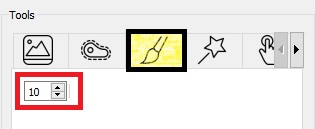
\includegraphics{Iconographie/brush_tool.jpg}		
\end{center}



\section{Region growing}

Cet outil permet une sélection semi-automatique des voxels en fonction de leur intensité (niveau de gris).

\begin{itemize}
	\item[\textbf{1}]: Selon le même principe que sous l'onglet Image tools, le double curseur permet de choisir les intensités minimale et maximale des voxels à sélectionner. Il suffira ensuite de cliquer sur la région d'intérêt de l'image pour voir apparaître la sélection. Cet outil est dynamique: une fois la sélection affichée, la modification des données (par changement des valeurs numériques ou déplacement des curseurs) permet de voir en temps réel les changements apportés à la sélection. Attention tout de même lors du travail en 3D qui nécessite un traitement d'un nombre plus importants de données et qui peut ralentir l'opération (cf infra).
	\item[\textbf{2}]: Ces options définissent le mode de sélection des voxels. De gauche à droite: travail en 2D (sur la coupe affichée) ou en 3D (sur toutes les coupes); la fonction Inside Label permet de choisir si la sélection en cours empiète ou non sur les labels enregistrés;la fonction connected permet de ne sélectionner que les voxels correspondants aux intensités choisies mais qui sont connectés les uns aux autres. Ainsi, désactiver l'option connected permet de sélectionner l'ensemble des points correspondants aux intensités choisies sur toute la coupe.	
	
	
\end{itemize}

\section{Landmarks}

Cet outil permet d'ajouter des points d'intérêt (landmarks) à votre image. Le bouton (+) permet l'ajout d'un point d'intérêt au niveau de la postion du curseur. (-) le supprime. Il est également possible de les importer ou les exporter.

\begin{center}
		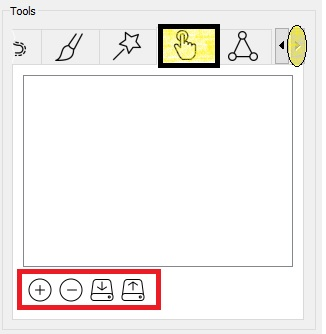
\includegraphics{Iconographie/landmarks.jpg}
\end{center}



\section{Mesh tools}

Cet outil permet de générer un maillage (objet 3D) à partir de votre segmentation.

\begin{center}
		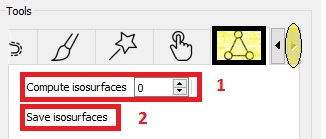
\includegraphics{Iconographie/mesh_tools.jpg}
\end{center}

\begin{itemize}
	\item[\textbf{1}]: Pour un label sélectionné, l'outil de calcul des surface permet de générer le maillage. La valeur numérique située à sa droite renseigne sur le nombre d'étapes de cette opération. Par convention, la valeur 0 équivaut à un calcul prenant en compte l'ensemble des données. Il est donc préférable de ne jamais changer cette valeur. Toute fois, si l'image à générer est trop volumineuse (génération d'un message d'erreur et fermeture du programme), il est possible de modifier cette valeur numérique. Il faudra alors choisir une valeur la plus élevée possible, qui correspond aux nombres de calculs effectués pour générer le maillage (exemple: 200).
	\item[\textbf{2}]: Une fois l'étape de calcul effectuée (peut prendre parfois quelques minutes), il est impératif de sauvegarder le maillage. Attention, le rendu 3D n'est pas visible sur MIST: pour le visionner, il faut utiliser un logiciel dédié (type Meshlab). Par précaution, nous vous conseillons d'ouvrir le maillage créé dans un logiciel dédié avant de fermer MIST pour prévenir des défauts de sauvegarde.

	
\end{itemize}

\part{Quelques exemples}

Nous avons vu l'ensemble des fonctionnalités de ce logiciel. La mise en application reste le meilleur moyen pour se les approprier. En voici quelques exemples.

\section{Segmenter la peau d'un sujet}

Un exemple intéressant permet de combiner plusieurs fonctionnalités du logiciel: segmenter la surface extérieure d'un sujet (peau).

Pour cela, charger l'image et débuter la segmentation en renommant un label par \og peau \fg , un autre par \og extérieur \fg et un dernier par \og interieur \fg . Sélectionner le label \og extérieur \fg . Grâce à l'outil \bsc{region growing}, cliquez sur l'air entourant votre sujet, puis ajustez le double curseur afin de n'obtenir la sélection que de l'extérieur. En pratique, cela équivaut à mettre le curseur de gauche au minimum, et faire varier le curseur de droite jusqu'à obtenir la sélection souhaitée. Pour enrigstrer ce choix, appuyer sur le bouton (+) ou la touche \bsc{enter}.

\begin{center}
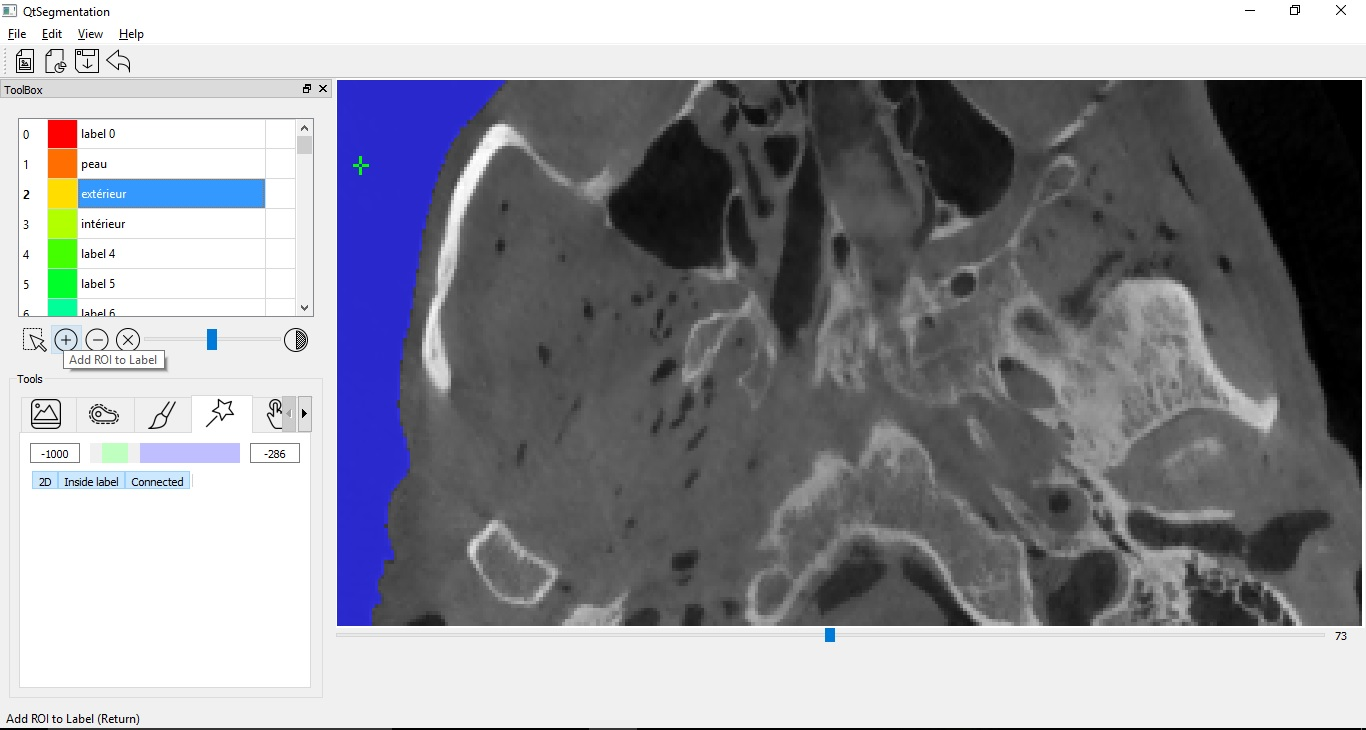
\includegraphics[scale=0.5]{Iconographie/Exemple_1_1.jpg}
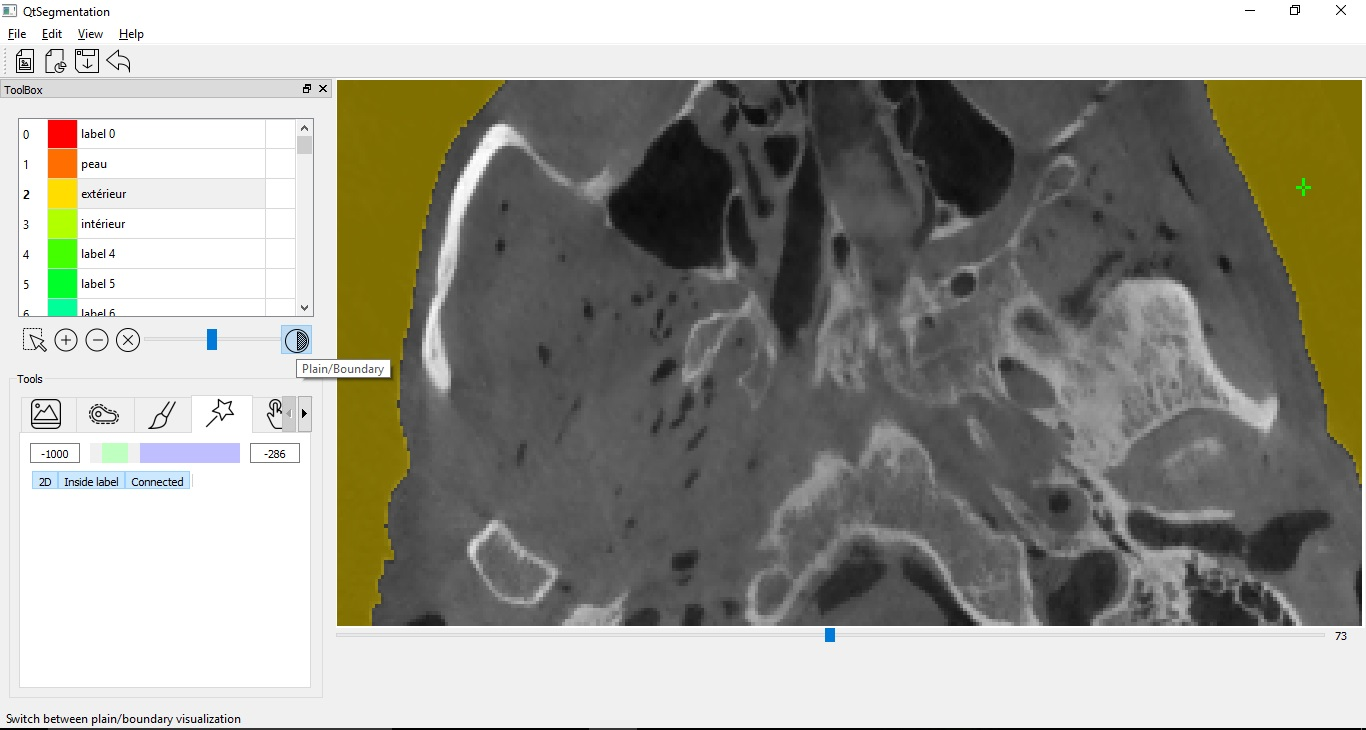
\includegraphics[scale=0.5]{Iconographie/Exemple_1_2.jpg}
\end{center}

Ensuite, resélectionnez le label \og exterieur \fg , grâce à l'icône de la flèche, puis dans \bsc{morphologicol operator}, cliquez sur invert. 

\begin{center}
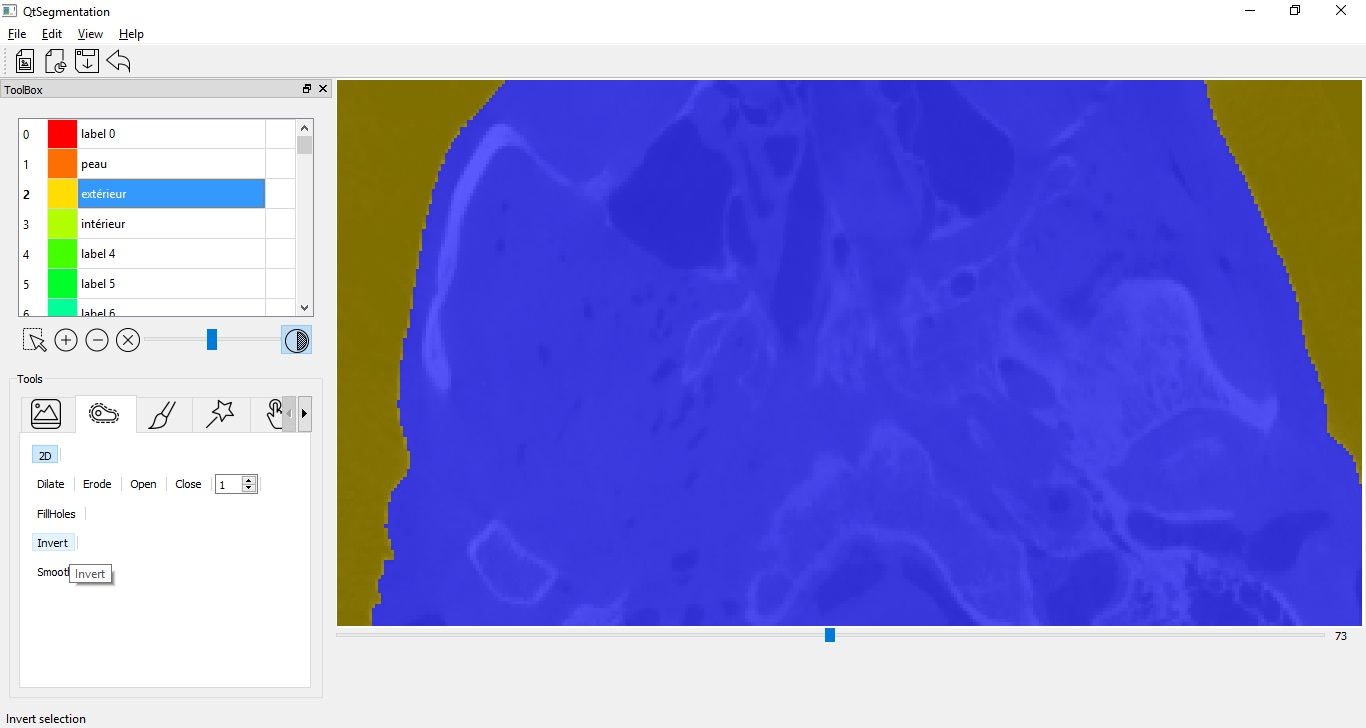
\includegraphics[scale=0.5]{Iconographie/Exemple_1_3.jpg}
\end{center}

Puis changez de label en cliquant sur l'intitulé du label \og intérieur \fg , et ajoutez la sélection à ce label (+) ou \bsc{enter}.

\begin{center}
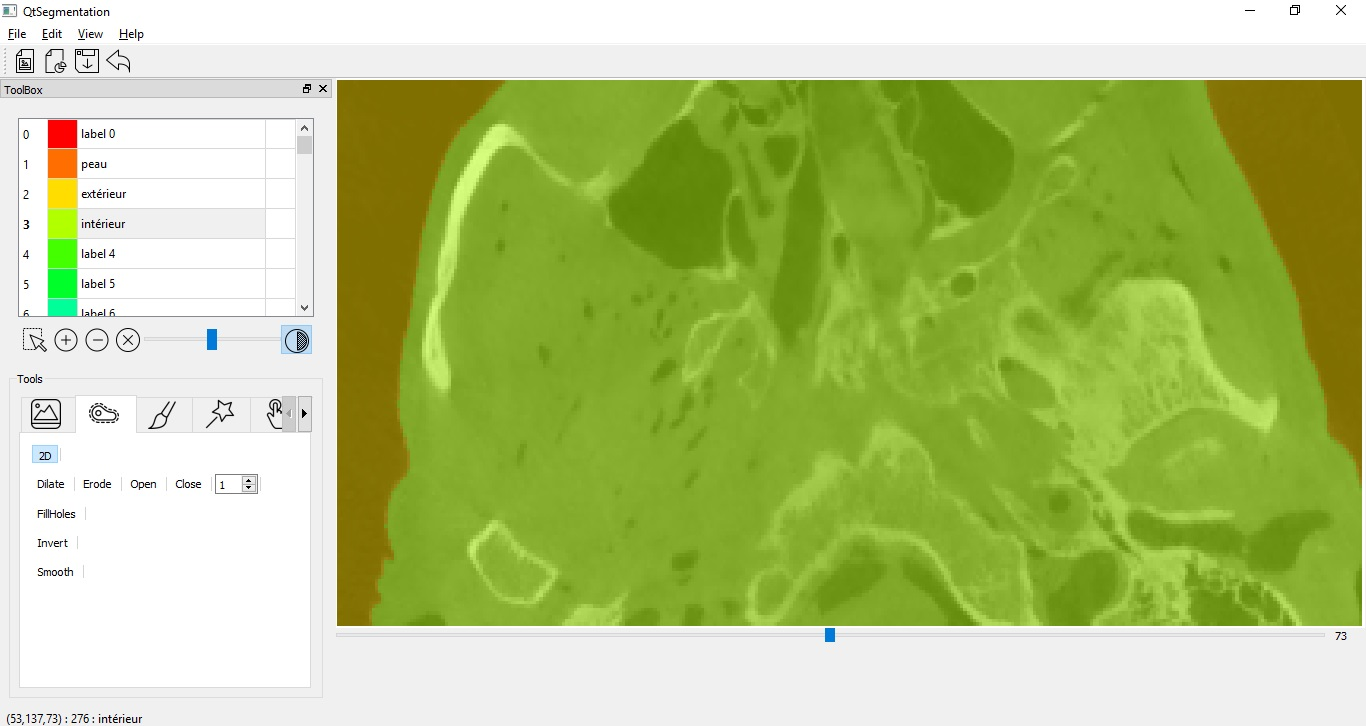
\includegraphics[scale=0.5]{Iconographie/Exemple_1_4.jpg}
\end{center}

Ensuite, resélectionnez le label \og intérieur \fg , grâce à l'icône de la flèche, puis dans \bsc{morphologicol operator}, cliquez sur dilate. Cela va dilater la sélection d'un voxel en partant du bord de l'image. Pour obtenir la peau, qui équivaut à une soustraction de votre nouvelle sélection par l'ancienne sélection ou autrement dit, qui correspond à la surface d'un pixel tout autour de l'ancienne sélection, il faut verrouiller le label \og intérieur \fg ,

\begin{center}
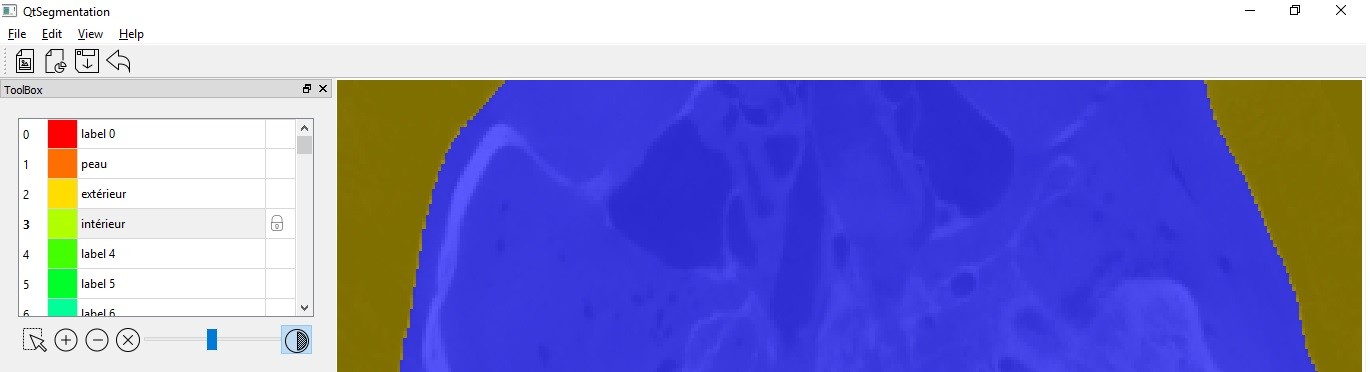
\includegraphics[scale=0.5]{Iconographie/Exemple_1_5.jpg}
\end{center}

puis sélectionner le label \og peau \fg et valider la sélection (+) ou \bsc{enter}.

Voici l'aspect final:

\begin{center}
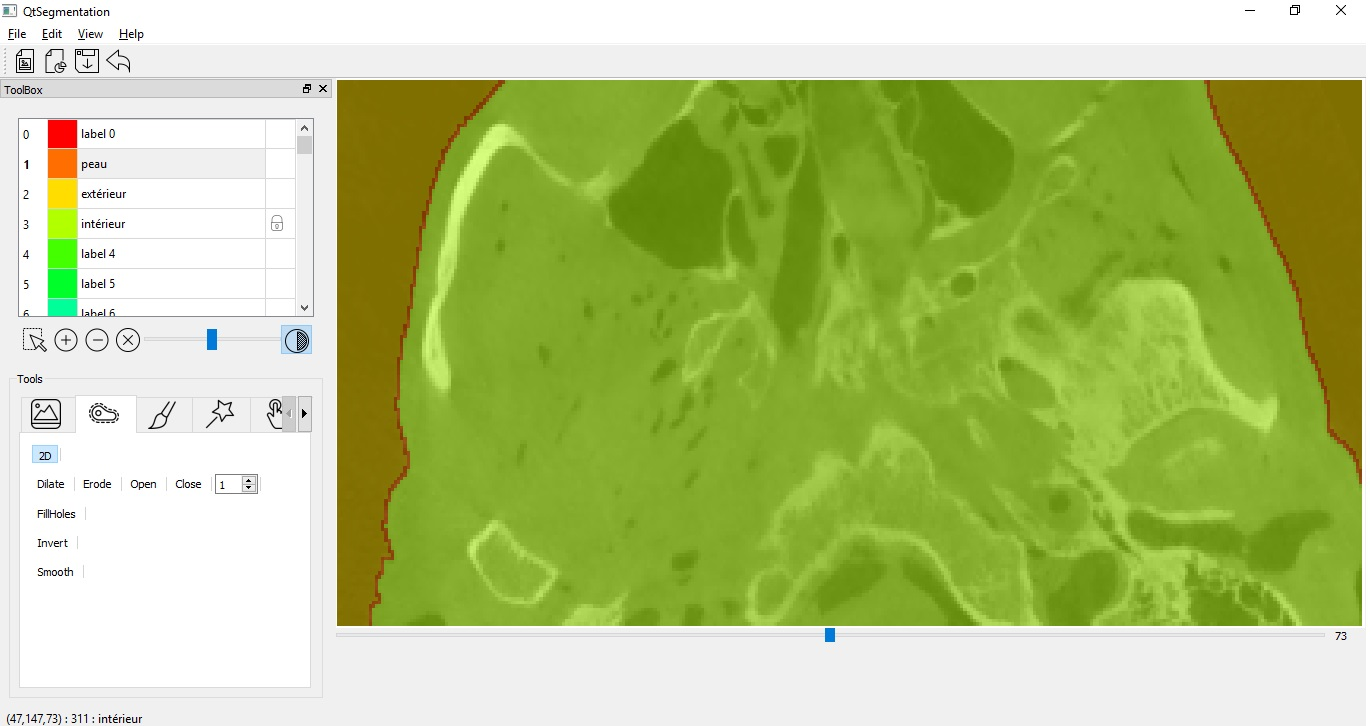
\includegraphics[scale=0.5]{Iconographie/Exemple_1_6.jpg}
\end{center}


Pour comprendre l'exemple: imaginez que MIST fonctionne comme les logiciels de retouche d'image, avec des calques. Chaque label représente un calque, et il faut trouver solution la plus simple et la moins chronophage pour aboutir à la segmentation souhaitée.	

Attention: la segmentation de la peau n'a été effectuée que sur cette coupe (car option 2D sélectionnée). Nous aurions pu réaliser ceci en 3D directement, mais cela peut occasionner des erreurs: si l'air extérieur est en contact avec l'air intérieur sur une ou plusieurs coupes, la sélection isolée de l'air extérieur n'aurait pas été possible en 3D! Cela aurait été le cas dans cet exemple puisque nous avions à faire à une tête humaine avec l'air communiquant par les narines. Pour pallier à ce problème, nous vous conseillons de réaliser la segmentation coupe par coupe au niveau de ces \og zones frontières \fg , puis de réaliser une segmentation 3D au dessus et en dessous de ces coupes.  

\newpage

\section{Epaissir une sélection contenant une cavité à respecter}

Si vous avez à segmenter une région d'intérêt contenant en son sein une cavité aérique qui ne doit pas apparaître dans votre sélection, voici un procédé. Dans le cas présenté, nous cherchons à sélectionner uniquement l'os au sein duquel se trouve un sinus aérien. Création des labels \og os \fg et \og sinus \fg . Grâce à l'outil \bsc{région growing}, sélectionner l'os et l'ajouter au label. A noter que contrairement à l'exemple précédent, le curseur de droite est à son maximum (densité osseuse), et l'on fait varier le curseur de gauche pour avoir la sélection souhaitée.

\begin{center}
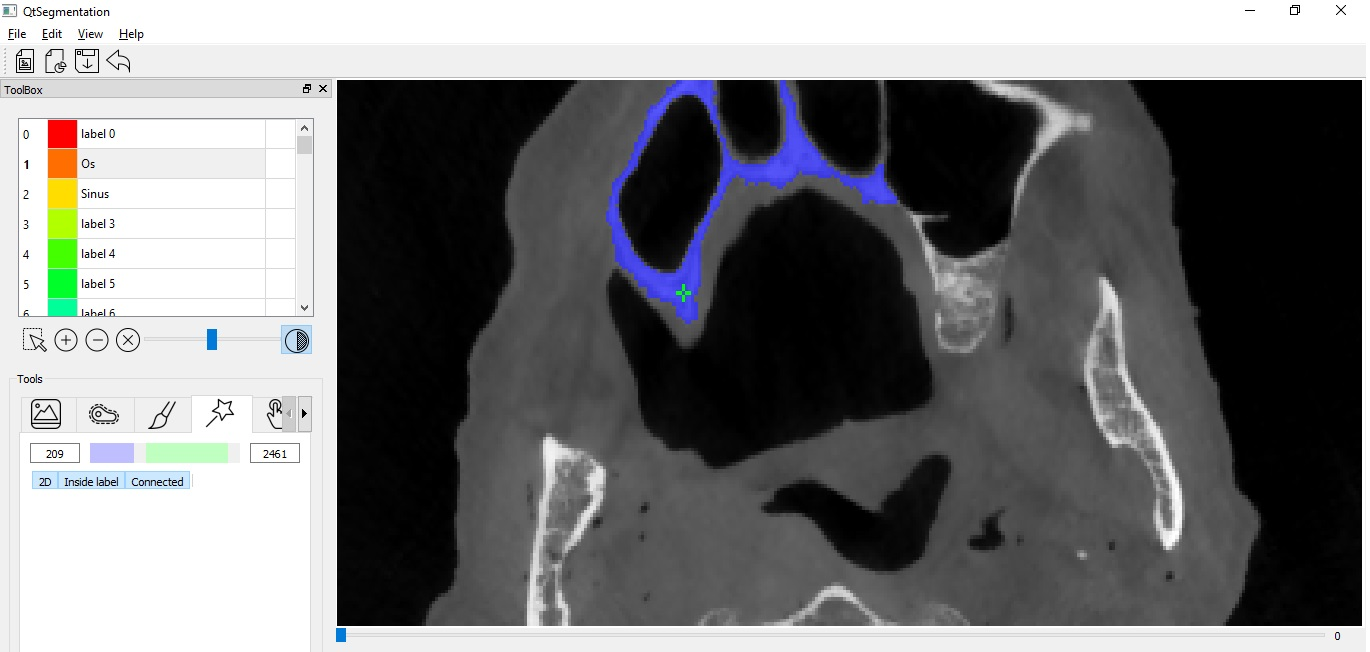
\includegraphics[scale=0.5]{Iconographie/Exemple_2_1.jpg}
\end{center}

Ensuite, avec le même outil, sélectionner l'air des sinus et l'ajouter au label \og sinus \fg .

\begin{center}
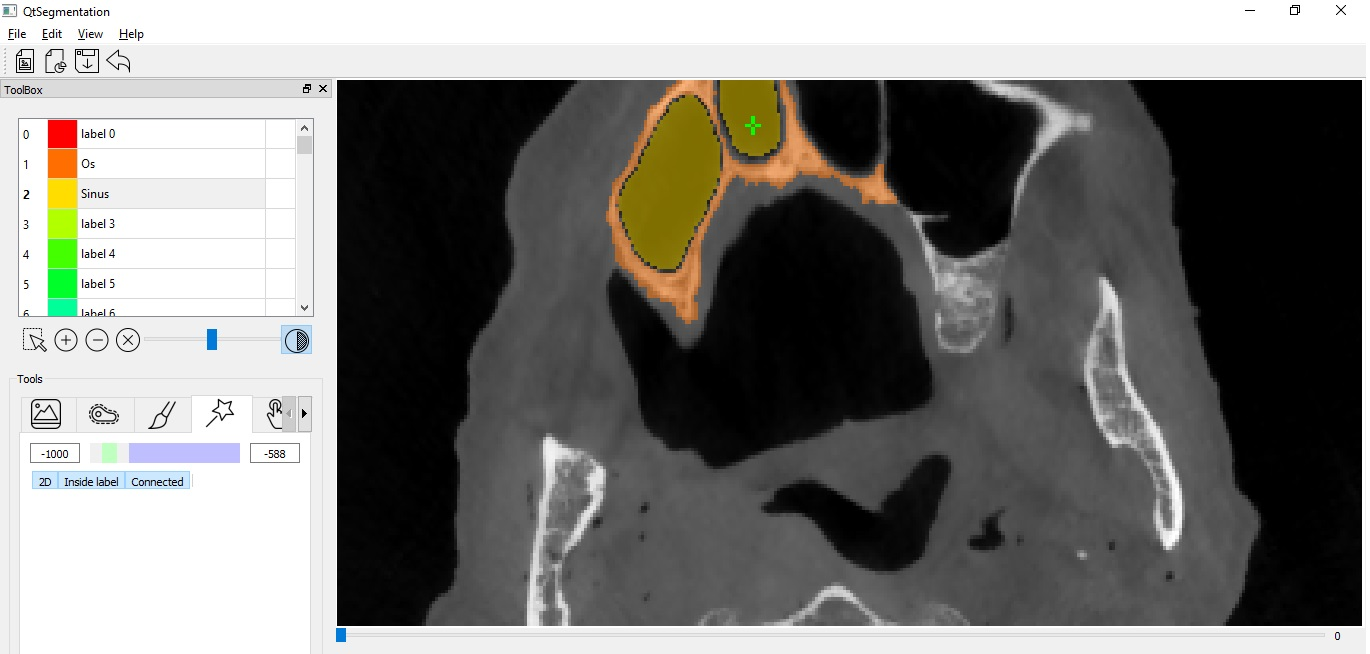
\includegraphics[scale=0.5]{Iconographie/Exemple_2_2.jpg}
\end{center}

La surface osseuse qui entoure les sinus est trop fine voire incomplète. Afin de l'épaissir, sans empiéter sur l'air sinusien, vérrouiller le label sinus, sélectionner le label os et dilater (\bsc{region growing}). Pour valider : (+) ou \bsc{enter}.

\begin{center}
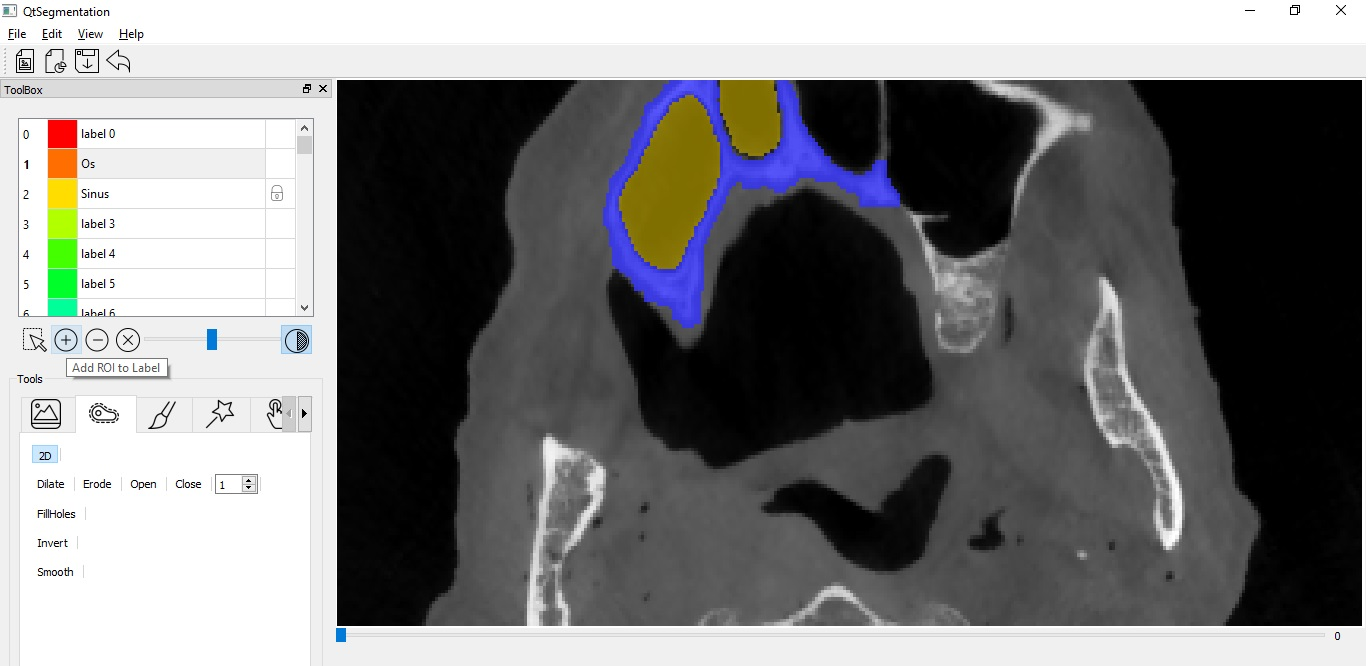
\includegraphics[scale=0.5]{Iconographie/Exemple_2_3.jpg}
\end{center}

Si vous n'êtes pas satisfait de la surface extérieure de votre label (trop crénelée), il est possible de procéder au lissage en sélectionnant votre label puis dans \bsc{region growing} et \bsc{smooth}. Procédez avec des répétitions d'étapes de lissage (en conservant la valeur numérique 1), pour appréhender les modifications apportées à la sélection.

\begin{center}
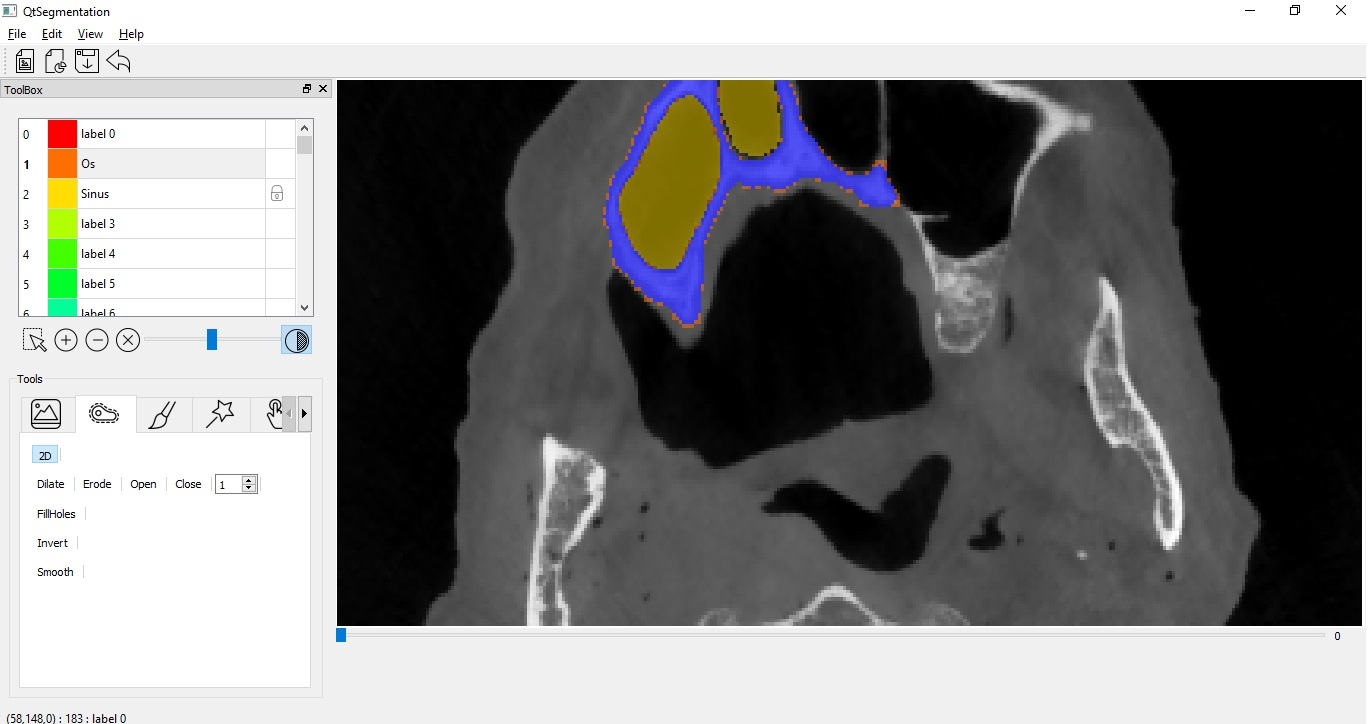
\includegraphics[scale=0.5]{Iconographie/Exemple_2_4.jpg}
\end{center}

Une fois la surface lissée à votre convenance (sélection en bleu, ancienne sélection de la couleur de votre label), il est nécessaire de réaliser une étape intermédiaire avant de l'ajouter à votre label (auquel cas, vous ajouteriez la nouvelle sélection à l'ancienne, ce qui équivaut à un retour au point de départ). 

\begin{center}
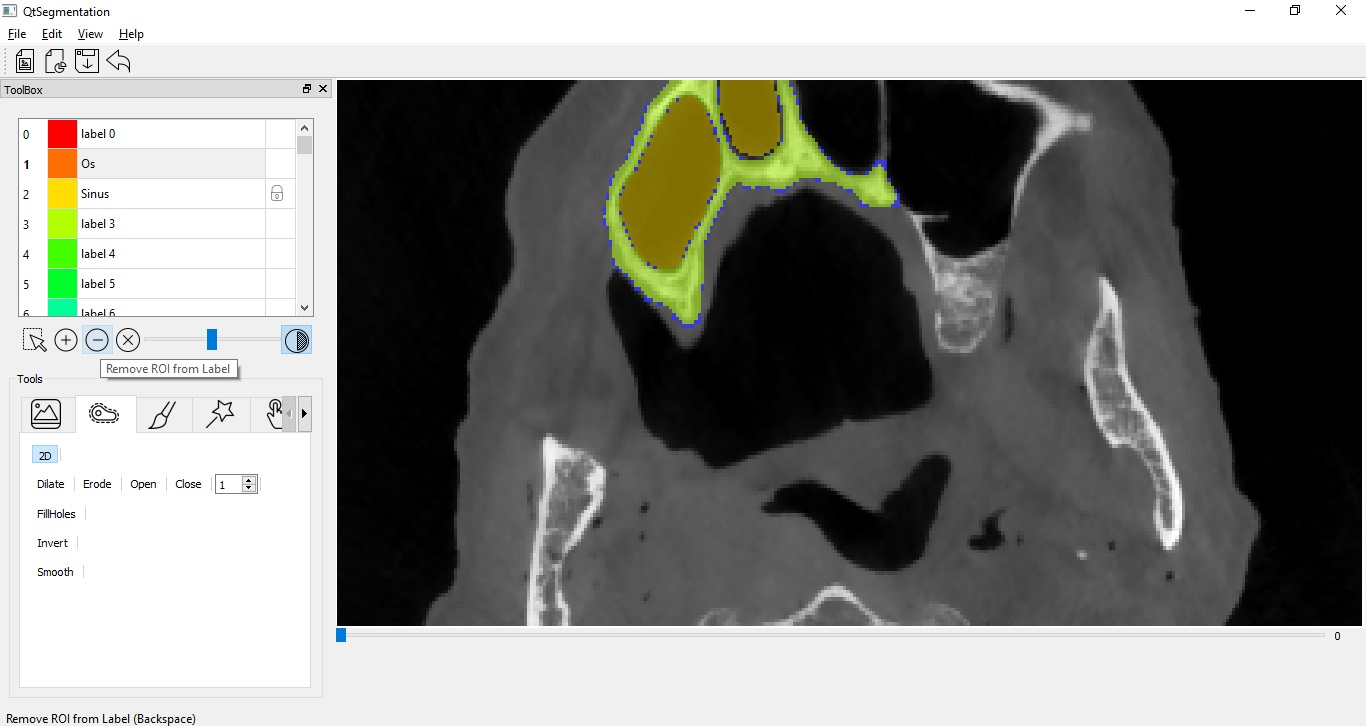
\includegraphics[scale=0.5]{Iconographie/Exemple_2_5.jpg}
\end{center}

Ajoutez donc votre sélection à un autre label (exemple \og label 3 \fg ), puis sélectionner de nouveau le label \og os \fg et supprimez-le (-) ou \bsc{return}. Ensuite, sélectionner le \og label 3 \fg et ajoutez le au label \og os \fg . Voici le rendu final.

\begin{center}
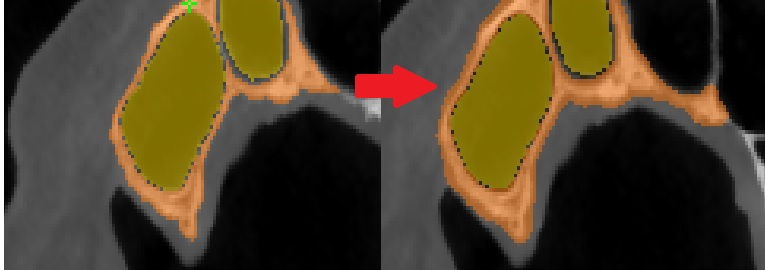
\includegraphics[scale=0.5]{Iconographie/Exemple_2_6.jpg}
\end{center}

\end{document}
